\documentclass[../main/thesis.tex]{subfiles}

\begin{document}
\section{Datasets}
This study combines different datasets consisting of fields from the Arome Arctic forecasting product and ice charts created by the Tromsø division of MET Norway.

\subsection{Sea Ice Charts}
The Sea Ice charts is an operational Sea Ice Concentration product provided by MET Norway. The product is manually drawn by a Sea Ice Specialist, and is distributed every workday at 15:00 UTC. The Sea Ice specialist assesses available SAR data from Sentinel 1 and Radarsat 2. However, due to the spatial variability in daily SAR coverage, visual, infrared and low resolution passive microwave observations are supplied to achieve a consistent spatial coverage \cite{MOI2015}. The Sea Ice charts are drawn in an ArcGIS production environment, and is as such intrinsically not projected onto a defined grid. Yet, the operational product available for download on \href{https://resources.marine.copernicus.eu/product-detail/SEAICE_ARC_SEAICE_L4_NRT_OBSERVATIONS_011_002/INFORMATION}{Copernicus} is provided as mean values on a 1km grid.

From the description of the Sea Ice charts given above, it is worth addressing the spatial inconsistency following the projection onto a uniformly sized grid. As the Sea Ice specialist draws polygons based on data from different satellite sources with a wide range of spatial resolution (80m from SAR, 1000m from visible / infrared and even lower resolution for passive microwave), the underlying uncertainty and detailed structures in the Sea Ice chart varies \cite{MOI2015}. Furthermore, I was made aware by one of the Sea Ice Analysts that time constraints also limits the hours different sections of the Ice chart is alloted. Moreover, the Sea Ice charts is an operational product aimed at end users in industries such as fishing, tourism, shipping or other maritime operations. This influences the decision-making when creating the final operational product. \todo{ask Trond on email}. As a consequence, the Sea Ice analyst spends approximately half of the total time draw polygons around the Svalbard archipelago. 

In conclusion, concerning the limited resources available both with regards to data availability as well as total hours available, the Sea Ice charts represents a dataset with a spatial uncertainty that is non-uniform across a single sample, and that changes in time. In spite of that, the involvement of a Sea Ice specialist which manually assures each Sea Ice charts, the temporal consistency as well as their high resolution has led us to believe that the Sea Ice charts is the overall best Sea Ice Concentration product available for the current study region.



\begin{figure}
    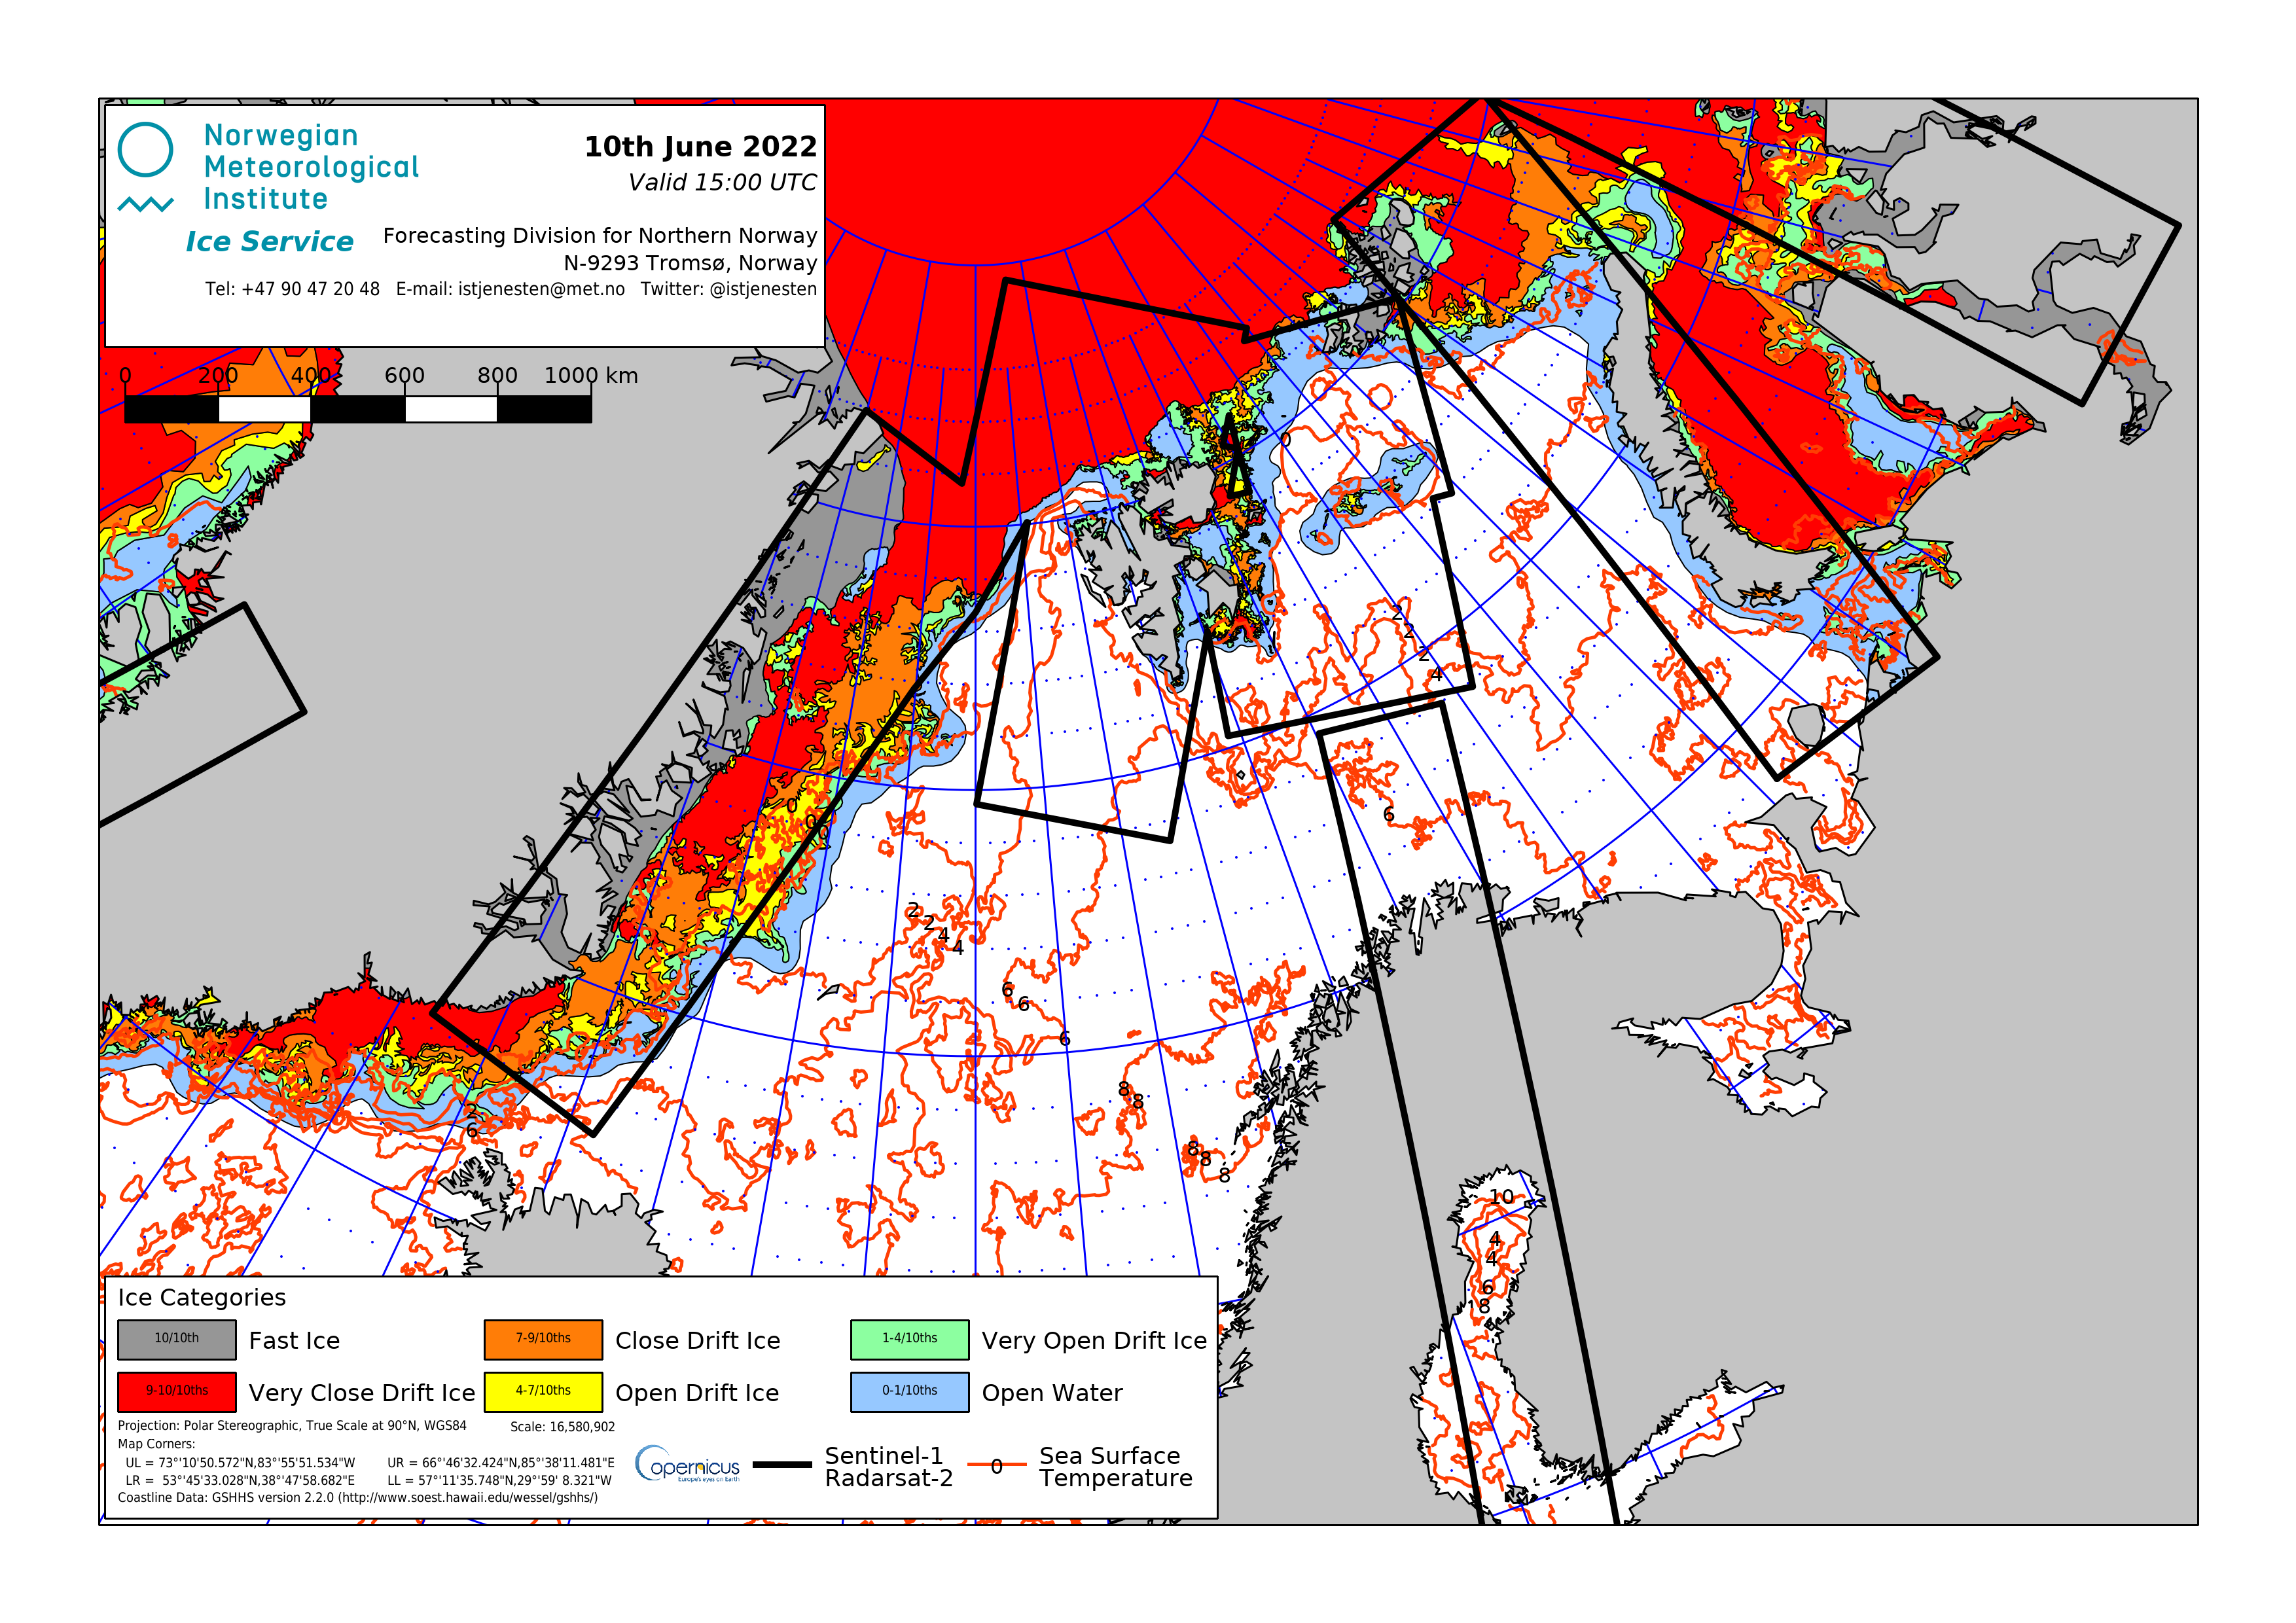
\includegraphics[width=\textwidth]{../figures/general_latest.png}
\end{figure}


% Local bibliography
\biblio

\end{document}